\myname{} is an extensible platform for enabling a variety of precision agriculture applications. In this section, we describe a case study of microclimate analysis application with our proposed architecture using a trace-driven simulation. 

    % \paragraph{Microclimate Analysis:} Agriculture researchers need high spatial resolution environmental data to investigate the impact of microclimates inside the tree canopy on the yield, diseases, pest attacks, and spread of unwanted insects and fungi~\cite{microclimates, microclimate-specifics, microcolimate-effect, microclimate-wsn}.
    
    % \paragraph{Apple Thinning:} Thinning is the process of removing a subset of apples from a tree early in the growth cycle, such that the remaining apples grow to a marketable size. There is a prior work on determining the amount of thinning spray needed to yield fruit of a particular size~\cite{thinning-history}, given the apple size and growth rate as the input~\cite{fruitlet-model}. This application requires high-resolution image capture of apple cluster images over time at a fixed angle~\cite{yield-prediction, crop-estimation}. It needs communication between different image capturing sources to combine the data for better sizing results. 
    % % It needs computational power at the edge to run computer vision algorithm to determine the size. 
     
    
    % \paragraph{Smart Insecticide Spraying:} Farmers attract insects to specific trees using pheromones and spray insecticide to kill the insects, a task that can be completed more efficiently if automated~\cite{ipm-scouting, ipm-overview, ipm-greenhouse}. An automated application would require autonomous release of the pheromones, make real-time inferences on the number of insects gathered, and finally initiating the release of insecticide spray. 

Our simulation environment uses a 100~Watt solar panel to harvest energy assuming the solar irradiation data obtained from Weather Station across 43 days of data  We analyze the power consumption of a mid-tier device with two major energy consuming components: 1) a Jetson Nano that consumes 2~Watts while idle, and 2) 3 power-hunger sensors that each consume 1~Watt when sampled (i.e. camera sensors) and take one minute to collectively sample data. First, a naive strategy polls for sensor data at high temporal resolution. In an adaptive strategy, we know the energy budget for the day, and decide on the polling rate for all the three sensors: the sampling period can be either moderate (10 minutes) or low (1 hour). The uptime is calculated for each day, for how many minutes in a day the device had energy and was able to collect readings. To understand potential data quaility, we compute how many hours were captured at what granularity.  

The key results are that for a naive strategy, we achieve an average up-time of 70\% compared to 90\% for the adaptive strategy. The adaptive strategy was able to reduce the "no data" periods from 37\% to 7\% by reducing the high resolution periods from 63\% to 54\%. 

\begin{figure}[t]
\centering
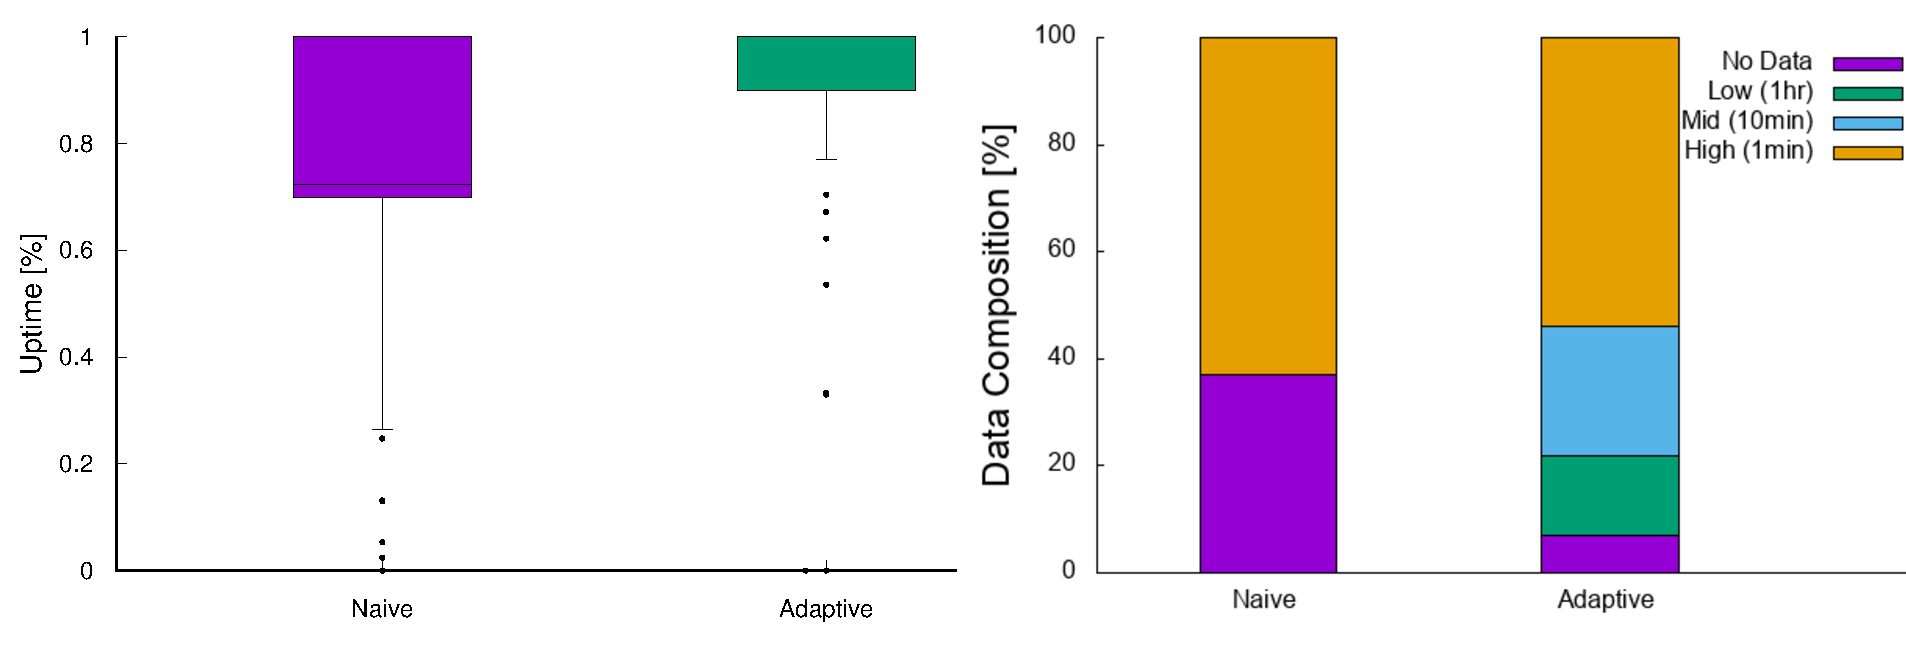
\includegraphics[width=0.4\textwidth]{./figures/combined.pdf}
% \vspace{-0.4cm}
\caption{Adaptive Sampling Results}
% \vspace{-0.3cm}
\label{fig:adaptive-sampling}
\end{figure}

Future application studies will incorporate the RFID hardware needed to sample the bottom tier sensors and perform analytics across the data they provide to account for redundant or missing data. Two other real-time applications we are exploring include:

 \noindent\textbf{Apple Thinning:} Thinning is the process of removing a subset of apples from a tree early in the growth cycle, such that the remaining apples grow to a marketable size. There is prior work in determining the amount of thinning spray needed to yield fruit of a particular size~\cite{thinning-history}, given the apple size and growth rate as the input~\cite{fruitlet-model}. This application requires high-resolution image capture of apple cluster images over time at a fixed angle~\cite{yield-prediction, crop-estimation}. Image data from different imagers needs to be combined to obtain images of sufficient quality.. 
    % % It needs computational power at the edge to run computer vision algorithm to determine the size. 
     
    
\noindent\textbf{Smart Insecticide Spraying:} Farmers attract insects to specific trees using pheromones and spray insecticide to kill the insects, a task that can be completed more efficiently if automated~\cite{ipm-scouting, ipm-overview, ipm-greenhouse}. An automated application would require autonomous release of the pheromones, make real-time inferences on the number of insects gathered, and finally initiating the release of insecticide spray. 